\documentclass[tikz,border=8pt]{standalone}
% Shared look for every TikZ diagram. Load with % Shared look for every TikZ diagram. Load with % Shared look for every TikZ diagram. Load with \input{../../tools/tikz-style.tex}
\usepackage[T1]{fontenc}
\usepackage{lmodern}
\renewcommand{\sfdefault}{lmr}  % diagrams use the same serif as the text
\usetikzlibrary{arrows.meta, positioning, shapes.geometric, calc, fit, backgrounds}
\definecolor{cblue}{HTML}{4C78A8}
\definecolor{corange}{HTML}{F58518}
\definecolor{cgreen}{HTML}{54A24B}
\definecolor{cred}{HTML}{E45756}
\definecolor{cpurple}{HTML}{B279A2}
\definecolor{cgrey}{HTML}{6B6B6B}
\tikzset{
  every picture/.style={font=\sffamily, line width=1.2pt},
  box/.style={draw=#1, fill=#1!12, rounded corners=4pt, align=center, inner sep=7pt, minimum height=1.1cm},
  box/.default=cgrey,
  arrow/.style={-{Stealth[length=3mm]}, draw=cgrey, line width=1.4pt},
  title/.style={font=\sffamily\bfseries\Large},
  note/.style={font=\sffamily\small, text=cgrey, align=center},
}
\AtBeginDocument{\hyphenpenalty=10000 \exhyphenpenalty=10000}

\usepackage[T1]{fontenc}
\usepackage{lmodern}
\renewcommand{\sfdefault}{lmr}  % diagrams use the same serif as the text
\usetikzlibrary{arrows.meta, positioning, shapes.geometric, calc, fit, backgrounds}
\definecolor{cblue}{HTML}{4C78A8}
\definecolor{corange}{HTML}{F58518}
\definecolor{cgreen}{HTML}{54A24B}
\definecolor{cred}{HTML}{E45756}
\definecolor{cpurple}{HTML}{B279A2}
\definecolor{cgrey}{HTML}{6B6B6B}
\tikzset{
  every picture/.style={font=\sffamily, line width=1.2pt},
  box/.style={draw=#1, fill=#1!12, rounded corners=4pt, align=center, inner sep=7pt, minimum height=1.1cm},
  box/.default=cgrey,
  arrow/.style={-{Stealth[length=3mm]}, draw=cgrey, line width=1.4pt},
  title/.style={font=\sffamily\bfseries\Large},
  note/.style={font=\sffamily\small, text=cgrey, align=center},
}
\AtBeginDocument{\hyphenpenalty=10000 \exhyphenpenalty=10000}

\usepackage[T1]{fontenc}
\usepackage{lmodern}
\renewcommand{\sfdefault}{lmr}  % diagrams use the same serif as the text
\usetikzlibrary{arrows.meta, positioning, shapes.geometric, calc, fit, backgrounds}
\definecolor{cblue}{HTML}{4C78A8}
\definecolor{corange}{HTML}{F58518}
\definecolor{cgreen}{HTML}{54A24B}
\definecolor{cred}{HTML}{E45756}
\definecolor{cpurple}{HTML}{B279A2}
\definecolor{cgrey}{HTML}{6B6B6B}
\tikzset{
  every picture/.style={font=\sffamily, line width=1.2pt},
  box/.style={draw=#1, fill=#1!12, rounded corners=4pt, align=center, inner sep=7pt, minimum height=1.1cm},
  box/.default=cgrey,
  arrow/.style={-{Stealth[length=3mm]}, draw=cgrey, line width=1.4pt},
  title/.style={font=\sffamily\bfseries\Large},
  note/.style={font=\sffamily\small, text=cgrey, align=center},
}
\AtBeginDocument{\hyphenpenalty=10000 \exhyphenpenalty=10000}

% cuboid: front-bottom-left corner (#1,#2), width #3, height #4, depth #5 (drawn up-right), colour #6
\newcommand{\cuboid}[6]{
  \fill[#6!18] (#1,#2) rectangle ++(#3,#4);
  \fill[#6!32] (#1,#2+#4) -- ++(#5*0.5,#5*0.4) -- ++(#3,0) -- ++(-#5*0.5,-#5*0.4) -- cycle;
  \fill[#6!45] (#1+#3,#2) -- ++(#5*0.5,#5*0.4) -- ++(0,#4) -- ++(-#5*0.5,-#5*0.4) -- cycle;
  \draw[#6, line width=1pt] (#1,#2) rectangle ++(#3,#4);
  \draw[#6, line width=1pt] (#1,#2+#4) -- ++(#5*0.5,#5*0.4) -- ++(#3,0) -- ++(0,-#4) -- ++(-#5*0.5,-#5*0.4);
  \draw[#6, line width=1pt] (#1+#3,#2+#4) -- ++(#5*0.5,#5*0.4);
}
\begin{document}
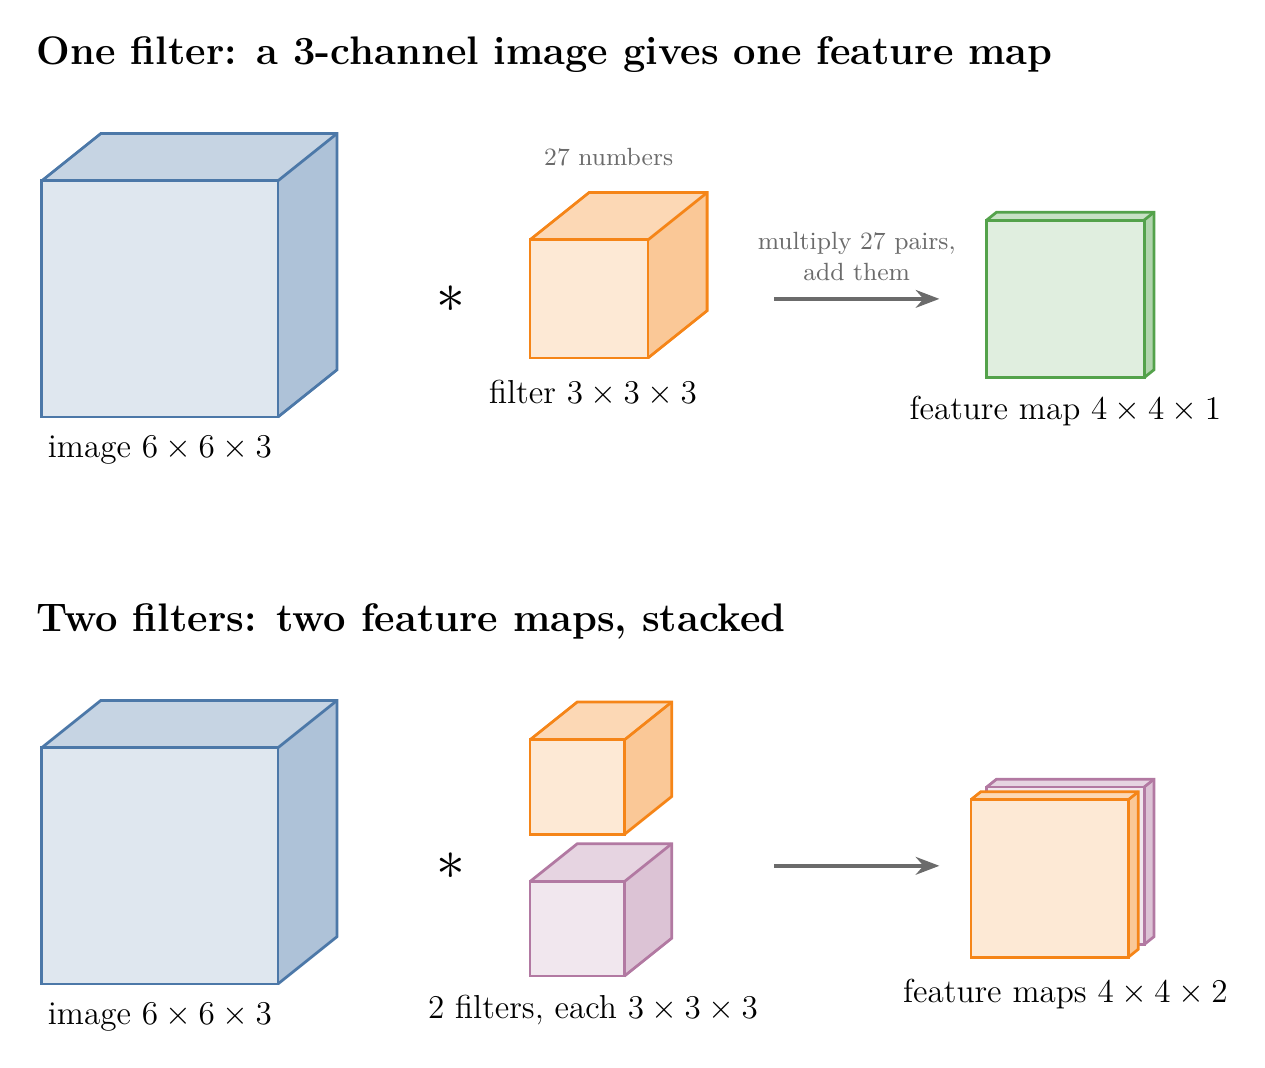
\begin{tikzpicture}[every node/.append style={font=\sffamily\large}]
  % one filter
  \node[title, anchor=west] at (-0.2,4.6) {One filter: a 3-channel image gives one feature map};
  \cuboid{0}{0}{3}{3}{1.5}{cblue}
  \node[below] at (1.5,-0.1) {image $6 \times 6 \times 3$};
  \node at (5.2,1.5) {\huge $*$};
  \cuboid{6.2}{0.75}{1.5}{1.5}{1.5}{corange}
  \node[below] at (7.0,0.6) {filter $3 \times 3 \times 3$};
  \node[note] at (7.2,3.3) {27 numbers};
  \draw[arrow] (9.3,1.5) -- (11.4,1.5);
  \node[note, above] at (10.35,1.6) {multiply 27 pairs,\\add them};
  \cuboid{12.0}{0.5}{2}{2}{0.25}{cgreen}
  \node[below] at (13.0,0.4) {feature map $4 \times 4 \times 1$};
  % two filters
  \begin{scope}[yshift=-7.2cm]
  \node[title, anchor=west] at (-0.2,4.6) {Two filters: two feature maps, stacked};
  \cuboid{0}{0}{3}{3}{1.5}{cblue}
  \node[below] at (1.5,-0.1) {image $6 \times 6 \times 3$};
  \node at (5.2,1.5) {\huge $*$};
  \cuboid{6.2}{1.9}{1.2}{1.2}{1.2}{corange}
  \cuboid{6.2}{0.1}{1.2}{1.2}{1.2}{cpurple}
  \node[below] at (7.0,0.0) {2 filters, each $3 \times 3 \times 3$};
  \draw[arrow] (9.3,1.5) -- (11.4,1.5);
  \cuboid{12.0}{0.5}{2}{2}{0.25}{cpurple}
  \cuboid{11.8}{0.34}{2}{2}{0.25}{corange}
  \node[below] at (13.0,0.2) {feature maps $4 \times 4 \times 2$};
  \end{scope}
\end{tikzpicture}
\end{document}
